
\documentclass[a4paper]{article}
\usepackage[OT1]{fontenc}
\usepackage{Sweave}
\usepackage[authoryear,round]{natbib}
\usepackage{fullpage}
\usepackage{verbatim}

\usepackage[a4paper, hmargin={2cm,2cm}, vmargin={2cm,2cm}]{geometry}


\bibliographystyle{ecology}

\DefineVerbatimEnvironment{Sinput}{Verbatim} {xleftmargin=2em}
\DefineVerbatimEnvironment{Soutput}{Verbatim}{xleftmargin=2em}
\DefineVerbatimEnvironment{Scode}{Verbatim}{xleftmargin=2em}
\fvset{listparameters={\setlength{\topsep}{0pt}}}
\renewenvironment{Schunk}{\vspace{\topsep}}{\vspace{\topsep}}

%%\VignetteIndexEntry{Species distributions}

\title{Modeling and mapping species distributions}
\author{Richard Chandler}


\begin{document}

\maketitle

\abstract{
A species' distribution can be characterized by either
occurrence probability or population density, defined for all
locations in some spatial domain. Defining distribution in terms of
these two parameters %These definitions of species distribution
avoids the ambiguity surrounding the indices of occurrence
or abundance produced by many presence-only algorithms. The
\texttt{unmarked} package contains methods of fitting
occurrence and abundance models, and can be used to
produce distribution maps with the help of \textbf{R}'s GIS
capabilities,
%, such as the \texttt{raster} package
%\citep{hijmans_vanEtten:2012}
as is demonstrated in this vignette.
Unlike many other tools for modeling
species distributions, the models in \texttt{unmarked} account for
bias due to spatial and temporal heterogeneity in detection
probability. Furthermore, \texttt{unmarked} includes models
of population dynamics, allowing one to map quantities
such as local colonization or extinction probability.
}




\section*{Mapping Occurrence Probability}



In this example, we fit the single-season occupancy model of
\citep{mackenzie_estimating_2002} to data on the European crossbill
(\emph{Loxia curvirostra}) collected in 267 1-km$^2$ sample
quadrats in Switzerland, 1999 \citep{schmid_etal:2004}.
We then use the model to compute the expected probability of
occurrence at each pixel in a raster defining the Swiss
landscape. %Computing confidence intervals for the predictions is also
%demonstrated, although the delta method approximation used is very
%time consuming when the number of pixels is high.

First we load the crossbill data, which is a list with two
components. The first component, \verb+crossbill+, is a data.frame
containing the
detection/non-detection data and some covariates such as the percent
cover of forest at each survey location. %The second component,
%\verb+switzerland+, is a list with two matrices defining the
%covariates: elevation and forest cover. Each matrix can be
%converted into a raster using the \texttt{raster} package. First, we
%format the crossbill data and fit the model. For additional details
The following commands format the data and fit the model using the
\verb+colext+ function. For more information
about this model, see the ``colext'' vignette that comes with
\texttt{unmarked}.


%\begin{comment}


\begin{Schunk}
\begin{Sinput}
> data(crossbill)
> umf <- unmarkedFrameOccu(
     y=as.matrix(crossbill[,c("det991", "det992", "det993")]),
     siteCovs=crossbill[,c("ele", "forest")],
     obsCovs=list(date=crossbill[,c("date991", "date992", "date993")]))
> sc <- scale(siteCovs(umf))
> siteCovs(umf) <- sc
> summary(umf)
\end{Sinput}
\begin{Soutput}
unmarkedFrame Object

267 sites
Maximum number of observations per site: 3 
Mean number of observations per site: 2.59 
Sites with at least one detection: 63 

Tabulation of y observations:
   0    1 <NA> 
 599   92  110 

Site-level covariates:
      ele               forest        
 Min.   :-1.46606   Min.   :-1.25551  
 1st Qu.:-0.99783   1st Qu.:-0.94836  
 Median :-0.06138   Median :-0.06307  
 Mean   : 0.00000   Mean   : 0.00000  
 3rd Qu.: 1.03115   3rd Qu.: 0.78610  
 Max.   : 2.43583   Max.   : 2.32182  

Observation-level covariates:
      date      
 Min.   : 10.0  
 1st Qu.: 40.0  
 Median : 59.0  
 Mean   : 57.3  
 3rd Qu.: 73.0  
 Max.   :115.0  
 NA's   :110    
\end{Soutput}
\end{Schunk}



Now we are ready to fit a model.

\begin{Schunk}
\begin{Sinput}
> (fm.occu <- occu(~date ~ele + I(ele^2) + forest, umf))
\end{Sinput}
\begin{Soutput}
Call:
occu(formula = ~date ~ ele + I(ele^2) + forest, data = umf)

Occupancy:
            Estimate    SE      z P(>|z|)
(Intercept)    0.464 0.541  0.857 0.39137
ele            1.228 0.319  3.846 0.00012
I(ele^2)      -1.333 0.417 -3.194 0.00140
forest         0.654 0.274  2.385 0.01706

Detection:
            Estimate      SE     z  P(>|z|)
(Intercept)  -2.2356 0.52283 -4.28 0.000019
date          0.0254 0.00752  3.39 0.000711

AIC: 455.3892 
\end{Soutput}
\end{Schunk}



Now that we have our fitted model, we can use the estimates to compute
the expected probability of occurrence at each pixel in the
landscape. The \verb+Switzerland+ dataset contains country-wide data.

\begin{Schunk}
\begin{Sinput}
> data(Switzerland)
> print(levelplot(elevation ~ x + y, Switzerland, aspect="iso",
                 col.regions=terrain.colors(100)))
\end{Sinput}
\end{Schunk}
\includegraphics{spp-dist-005}

The \texttt{raster} package \citep{hijmans_vanEtten:2012}
makes this easy. Here are the
commands to create raster objects from the covariate matrices that
come with the crossbill data.

\begin{Schunk}
\begin{Sinput}
> library(raster)
> elevation <- rasterFromXYZ(Switzerland[,c("x","y","elevation")],
     crs="+proj=somerc +lat_0=46.95240555555556 +lon_0=7.439583333333333 +k_0=1 +x_0=600000 +y_0=200000 +ellps=bessel +towgs84=674.374,15.056,405.346,0,0,0,0 +units=m +no_defs")
> forest <- rasterFromXYZ(Switzerland[,c("x","y","forest")],
     crs="+proj=somerc +lat_0=46.95240555555556 +lon_0=7.439583333333333 +k_0=1 +x_0=600000 +y_0=200000 +ellps=bessel +towgs84=674.374,15.056,405.346,0,0,0,0 +units=m +no_defs")
\end{Sinput}
\end{Schunk}


\begin{Schunk}
\begin{Sinput}
> attr(sc, "scaled:center")
\end{Sinput}
\begin{Soutput}
       ele     forest 
1189.32584   34.74532 
\end{Soutput}
\begin{Sinput}
> attr(sc, "scaled:scale")
\end{Sinput}
\begin{Soutput}
      ele    forest 
640.71471  27.67431 
\end{Soutput}
\begin{Sinput}
> ele.s <- (elevation-1189)/640
> forest.s <- (forest-34.7)/27.7
> ef <- stack(ele.s, forest.s)
> layerNames(ef) <- c("ele", "forest")
> plot(ef, col=terrain.colors(100))
\end{Sinput}
\end{Schunk}
\includegraphics{spp-dist-007}



The reason for assigning the layerNames is that the
\verb+predict+ function, which will be used shortly, requires that the
rasters have names identical to the names of the variables used in
the model fitting process.

The \verb+predict+ function is useful for computing
spatially-referenced model predictions, standard errors, and
confidence intervals, but it is computationally demanding when
there are many pixels in the raster. Thus, if measures of uncertainty
are not
required, the following code can be used to quickly produce the species
distribution map shown in Fig.\ref{fig:psi1}.

\begin{Schunk}
\begin{Sinput}
> (beta <- coef(fm.occu, type="state"))
\end{Sinput}
\begin{Soutput}
     psi(Int)      psi(ele) psi(I(ele^2))   psi(forest) 
    0.4638233     1.2276426    -1.3327186     0.6544976 
\end{Soutput}
\begin{Sinput}
> logit.psi <- beta[1] + beta[2]*ele.s + beta[3]*ele.s^2 + beta[4]*forest.s
> psi <- exp(logit.psi) / (1 + exp(logit.psi))
> #plot(psi, col=terrain.colors(100))
> print(spplot(psi, col.regions=terrain.colors(100)))
\end{Sinput}
\end{Schunk}

\begin{figure}
  \includegraphics[width=6in,height=3in]{spp-dist-psi}
  \caption{A species distribution map for the European crossbill in
    Switzerland for the year 1999. The colors represent the probability
    of occurrence.}
\label{fig:psi1}
\end{figure}

The same can be done for any other parameter. For example, if we
modeled density, perhaps using the \verb+distsamp+ function, we could
compute the expected number of individuals in each pixel. Another
option with the crossbill data is to map expected colonization
probabilities, which can be accomplished using the following code.


As of version 0.9-6, the \verb+predict+ method in \texttt{unmarked}
can make predictions using an object of class \verb+RasterStack+ from the
\texttt{raster} package. As mentioned previously, the rasters must be
named, perhaps by using the \verb+layerNames(someraster) <- somename+
method. The object
returned by \verb+predict+ is another raster stack with rasters for
the expected values of the parameter of interest, the standard errors,
and the upper and lower confidence intervals. The following example
is very slow because there are many of pixels in the raster. The
resulting map is shown in Fig.\ref{fig:predict}.

\begin{Schunk}
\begin{Sinput}
> rasters <- stack(elevation, forest)
> E.psi <- predict(fm, type="psi", newdata=rasters)
\end{Sinput}
\begin{Sinput}
> plot(E.psi, axes=FALSE)
\end{Sinput}
\end{Schunk}
\begin{figure}[b!]
  \centering
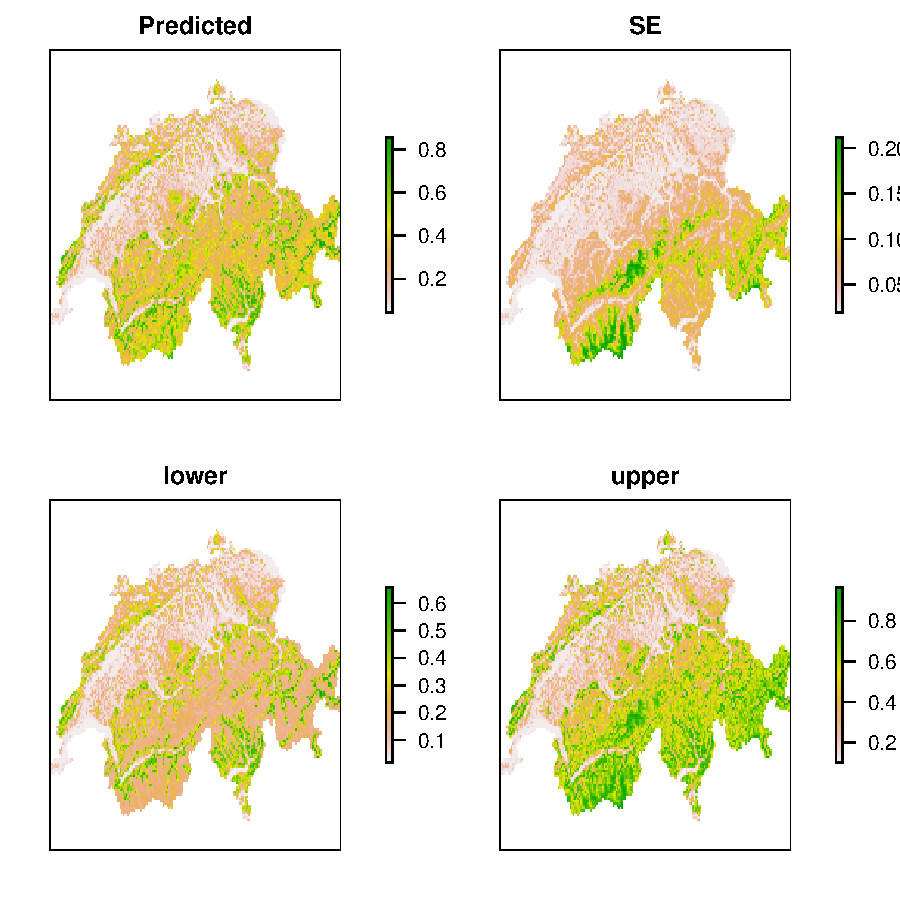
\includegraphics[width=5in,height=5in]{spp-dist-predict}
\caption{Expected occurrence probability along with standard errors
  and the limits of the asymptotic 95\% confidence interval.}
\label{fig:predict}
\end{figure}

Users should be cautious when predicting from models that have
categorical predictor variables, \emph{i.e.} \verb+factor+s. The
\texttt{raster} package does not have advanced methods for handling
factors, and thus it is not easy to automatically create dummy
variables from them as can typically be done using
\verb+model.matrix+. The safest option is to create the dummy
variables manually before fitting the models, and to use the same
variables as rasters for prediction.



%\end{comment}




\section*{Mapping Population Density}

Although distribution is typically described in terms of
ocurrence probability, density is a better descriptor for several
reasons. First, density can be readily converted to abundance for any
region of interest; whereas occurrence probability does not scale with
area.



\begin{Schunk}
\begin{Sinput}
> data(issj)
> data(cruz)
> elev <- rasterFromXYZ(cruz[,c("x","y","elevation")],
      crs="+proj=utm +zone=11 +ellps=GRS80 +datum=NAD83 +units=m +no_defs")
> #plot(elev, col=terrain.colors(100))
> #points(issj[,c("x","y")], cex=0.5)
> 
> print(
 wireframe(elevation ~ x + y, cruz, drape=TRUE,
           screen=list(z=10, x=-10),
           aspect=0.5, xlab="", ylab="", zlab="",
 #          xlim=c(229900,267000), ylim=c(3762000,3770000),
           par.settings = list(axis.line = list(col = "transparent")),
           par.box = c(col = "transparent"),
           col.regions=terrain.colors(100),
           colorkey=FALSE)
 )
> 
\end{Sinput}
\end{Schunk}
\includegraphics{spp-dist-010}




\begin{Schunk}
\begin{Sinput}
> covs <- scale(issj[,c("elevation", "forest", "chaparral")])
> area <- pi*300^2 / 10000
> jayumf <- unmarkedFrameDS(y=as.matrix(issj[,1:3]),
                           siteCovs=data.frame(covs, area),
                           dist.breaks=c(0,100,200,300),
                           unitsIn="m", survey="point")
> head(jayumf)
\end{Sinput}
\begin{Soutput}
Data frame representation of unmarkedFrame object.
   y.1 y.2 y.3   elevation     forest  chaparral     area
1    0   0   2 -1.20607849 -0.3309618 -0.1218243 28.27433
2    0   0   0 -0.36132054 -0.4429552  0.8384709 28.27433
3    0   0   0 -0.45797193 -0.3738751  2.1319298 28.27433
4    0   0   0 -0.14196112  1.3908065 -0.2737078 28.27433
5    0   0   0 -0.72588125 -0.4869152 -1.1562240 28.27433
6    0   0   0  0.01704522  0.6706992  0.2989173 28.27433
7    0   0   0 -0.11866710 -0.2671150  1.0326122 28.27433
8    0   0   0 -0.76411740 -0.4921486 -0.9332983 28.27433
9    0   0   0  0.40065595  0.5440524 -1.0759952 28.27433
10   0   0   0 -0.24030211 -0.4921486 -1.1023299 28.27433
\end{Soutput}
\begin{Sinput}
> fm1 <- distsamp(~chaparral ~chaparral + elevation + offset(log(area)),
                 jayumf, output="abund")
> fm1
\end{Sinput}
\begin{Soutput}
Call:
distsamp(formula = ~chaparral ~ chaparral + elevation + offset(log(area)), 
    data = jayumf, output = "abund")

Abundance:
            Estimate     SE      z  P(>|z|)
(Intercept)   -2.827 0.1609 -17.57 4.33e-69
chaparral      0.957 0.1460   6.55 5.60e-11
elevation     -0.244 0.0932  -2.61 8.96e-03

Detection:
                 Estimate     SE     z  P(>|z|)
sigma(Intercept)     4.73 0.0845 55.96 0.000000
sigmachaparral      -0.25 0.0744 -3.36 0.000773

AIC: 964.6426 
\end{Soutput}
\begin{Sinput}
> 
\end{Sinput}
\end{Schunk}

\begin{Schunk}
\begin{Sinput}
> elev <- rasterFromXYZ(cruz[,c("x","y","elevation")],
      crs="+proj=utm +zone=11 +ellps=GRS80 +datum=NAD83 +units=m +no_defs")
> forest <- rasterFromXYZ(cruz[,c("x","y","forest")],
      crs="+proj=utm +zone=11 +ellps=GRS80 +datum=NAD83 +units=m +no_defs")
> chap <- rasterFromXYZ(cruz[,c("x","y","chaparral")],
      crs="+proj=utm +zone=11 +ellps=GRS80 +datum=NAD83 +units=m +no_defs")
> area.raster <- chap
> values(area.raster) <- 300*300/10000 # area of a grid pixel
> attr(covs, "scaled:center")
\end{Sinput}
\begin{Soutput}
  elevation      forest   chaparral 
202.0023616   0.0673357   0.2703592 
\end{Soutput}
\begin{Sinput}
> attr(covs, "scaled:scale")
\end{Sinput}
\begin{Soutput}
  elevation      forest   chaparral 
124.8818069   0.1368199   0.2338295 
\end{Soutput}
\begin{Sinput}
> elev.s <- (elev-202)/125
> forest.s <- (forest-0.0673)/0.137
> chap.s <- (chap-0.270)/0.234
> habitat <- stack(elev.s, forest.s, chap.s, area.raster)
> layerNames(habitat) <- c("elevation", "forest", "chaparral", "area")
> 
> 
\end{Sinput}
\end{Schunk}




\begin{Schunk}
\begin{Sinput}
> E <- predict(fm1, type="state", newdata=habitat)
\end{Sinput}
\begin{Soutput}
  doing row 1000 of 5625 rows
  doing row 2000 of 5625 rows
  doing row 3000 of 5625 rows
  doing row 4000 of 5625 rows
  doing row 5000 of 5625 rows
\end{Soutput}
\begin{Sinput}
> plot(E)
> cellStats(E[["Predicted"]], "sum")
\end{Sinput}
\begin{Soutput}
[1] 932.9886
\end{Soutput}
\begin{Sinput}
> 
\end{Sinput}
\end{Schunk}
\includegraphics{spp-dist-013}









\newpage

\bibliography{unmarked}

\end{document}
